\chapter{Základné pojmy a predošlé výsledky}

V tejto kapitole si zavedieme pojmy a označenia, ktoré budeme používať
vo zvyšku práce. Taktiež si podrobne popíšeme predošlé výsledky o
$L(2,1)$-farbeniach grafov.

\section{Základné pojmy}

Pokiaľ nebude povedané inak, grafy spomínané v tejto práci budú neorientované,
súvislé a jednoduché, bez slučiek a násobných hrán. Množinu vrcholov budeme
označovať $V(G)$ a množinu hrán $E(G)$. Vzdialenosť dvoch vrcholov $u$ a $v$
v grafe $G$ budeme označovať $d_G(u,v)$. Pokiaľ bude z kontextu jasné, o
ktorý graf sa jedná, budeme vzdialenosť vrcholov $u, v$ značiť $d(u,v)$.

Pre ľubovoľný vrchol $v$ budeme symbolom $N(v)$ značiť množinu vrcholov, ktoré
sú hranou spojené s $v$. Pod značením $N[v]$ budeme rozumieť množinu $N(v) \cup \{v\}$.
Toto značenie rozšírime aj na množiny vrcholov. Pre množinu vrcholov $S$ budeme
symbolom $N[S]$ značiť množinu $\bigcup \limits_{v \in S} N[v]$ a symbolom
$N(S)$ označíme množinu $N[S] - S$.

Ako prvé si poriadne
zadefinujeme $L(2,1)$-farbenie grafu a problémy s ním súvisiace.

\begin{defn}
    $L(2,1)$-farbenie grafu $G$ je zobrazenie $\omega : V(G) \to \mathbb{N}$,
    ktoré spĺňa nasledujúce podmienky:

    \begin{itemize}
        \item $\forall u, v \in V(G): d(u, v) = 1 \Rightarrow \left| \omega(u) - \omega(v) \right| \ge 2$,
        \item $\forall u, v \in V(G): d(u, v) = 2 \Rightarrow \omega(u) \neq \omega(v)$.
    \end{itemize}
\end{defn}

Pri obyčajných vrcholových, či hranových farbeniach grafov skúmame, aký
najmenší počet farieb potrebujeme pre platné ofarbenie daného grafu. Podobne
si vieme pri $L(2,1)$-farbeniach všímať, aké najväčšie číslo používajú. Toto
číslo budeme nazývať \emph{rozpätím $L(2,1)$-farbenia}. Najmenšie možné rozpätie
$L(2,1)$-farbenia grafu $G$ budeme nazývať \emph{$L(2,1)$-farbiace číslo} a
označovať $\lambda(G)$. Všimnime si, že $L(2,1)$-farbenie s
rozpätím $k$ môže používať až $k+1$ rôznych hodnôt.

\begin{defn}
    Pod problémom $L(2,1)$-farbenia budeme rozumieť nasledujúci rozhodovací problém.
    Inštanciou je graf $G$ a prirodzené číslo $k$. Inštancia je riešiteľná práve vtedy,
    ak existuje $L(2,1)$-farbenie grafu $G$ s rozsahom $k$.
\end{defn}

Podobne by sme mohli zadefinovať problém rozpätia $L(2,1)$-farbenia, v ktorom by sme
pre daný graf hľadali jeho farbiace číslo. Pre každý graf existuje triviálne ofarbenie
používajúce párne čísla od $0$ po $2n - 2$, z hľadiska výpočtovej zložitosti
sú teda tieto problémy takmer totožné.

V práci budeme často používať pojem \emph{čiastočného $L(2,1)$-farbenia}, preto
si ho poriadne zadefinujeme.

\begin{defn}
    Nech $G$ je graf, nech $S$ je podmnožina vrcholov grafu $G$. Pod pojmom
    čiastočné $L(2,1)$-farbenie množiny $S$ v grafe $G$ budeme rozumieť zobrazenie
    $\omega : S \to \mathbb{N}$, ktoré spĺňa nasledujúce podmienky:

    \begin{itemize}
        \item $\forall u, v \in S: d_G(u,v) = 1 \Rightarrow \left| \omega(u) - \omega(v) \right| \ge 2$,
        \item $\forall u, v \in S: d_G(u,v) = 2 \Rightarrow \omega(u) \neq \omega(v)$.
    \end{itemize}

    Pojmom čiastočné $L(2,1)$-farbenie grafu $G$ budeme označovať čiastočné farbenie
    niektorej podmnožiny jeho vrcholov.
\end{defn}

\section{Predošlé výsledky}

Veľkou oblasťou skúmania $L(2,1)$-farbení boli dolné a horné ohraničenia na hodnotu $\lambda(G)$.
Vhodnou charakteristikou sa ukázal byť maximálny stupeň grafu. Pre všeobecné
grafy bolo najprv dokázané horné ohraničenie $\lambda(G) \leq \Delta^2 + 2\Delta$
pomocou jednoduchého pažravého priradenia\cite{griggs_yeh_tree},
ktoré bolo neskôr vylepšené na $\lambda(G) \leq \Delta^2 + \Delta$ s použitím
šikovnejšieho priradzovania\cite{chang_kuo}.

Pre špeciálne triedy grafov sa podarilo dokázať silnejšie ohraničenia. Napríklad
pre grafy s priemerom $2$ platí a je tesný odhad $\lambda(G) \leq \Delta^2$\cite{griggs_yeh_tree}.
Ďalej pre chordálne grafy platí odhad $\lambda(G) \leq \frac{\left( \Delta + 3 \right)^2}{4}$\cite{griggs_yeh_tree}.

Medzi ďalšie triedy grafov, na ktorých sú dokázané tesnejšie obmedzenia na $L(2,1)$-farbiace
číslo, patria aj stromy s obmedzením $\Delta + 1 \leq \lambda(G) \leq \Delta + 2$\cite{griggs_yeh_tree},
kaktusy s obmedzením $\Delta + 1 \leq \lambda(G) \leq \Delta + 3$\cite{kaktusy} a vonkajšie planárne
grafy s obmedzením $\Delta + 1 \leq \lambda(G) \leq \Delta + 8$\cite{outer_planar_bound}.

Griggs a Yeh taktiež vyslovili hypotézu, že v každom grafe platí $\lambda(G) \leq \Delta^2$,
ktorá dodnes nebola vyriešená.

Ďalej sa pozrieme na zopár tried grafov, na ktorých vieme riešiť problém $L(2,1)$-farbenia
v polynomiálnom čase a popíšeme si zodpovedajúce algoritmy.

\section{Polynomiálne farbenie špeciálnych grafov}

Prvou triedou grafov, pre ktoré bol objavený polynomiálny algoritmus na riešenie
problému $k$-$L(2,1)$-farbenia, sú stromy\cite{chang_kuo}. Tento algoritmus si
podrobne popíšeme.

\subsection{Chang-Kuo algoritmus}

Vstupom pre algoritmus je strom $T$ zakorenený v listovom vrchole so synom $r$ a číslo $k$.
Tento algoritmus zistí, či existuje $L(2,1)$-farbenie grafu $T$ s rozpätím $k$.

Pre ľubovoľný
vrchol $v$ zadefinujeme $T(v)$ ako podstrom stromu $T$ zakorenený vo vrchole $v$. Taktiež
zadefinujeme $T'(v')$ ako $T(v)$ s novým vrcholom $v'$, ktorý je spojený iba s $v$, čiže
$$ G\left(V(T(v)) \cup \{ v' \}, E(T(v)) \cup \{ (v', v)\} \right) $$
kde $v'$ je nový vrchol nevyskytujúci sa v $T(v)$.

Základnou myšlienkou algoritmu je konštruovať množiny $S(T(v))$ definované nasledovne:
$$S(T(v)) = \{ (a, b) | \textrm{ existuje } L(2,1) \textrm{ farbenie } f \textrm{ grafu } T'(v') \textrm{ také, že } f(v) = a \textrm{ a } f(v') = b\}$$

Pre ľubovoľný listový vrchol $v_l$ ľahko vidíme, že 
$$S(T(v_l)) = \{ (a, b) | a \leq k \wedge b \leq k \wedge |a - b| \ge 2\}$$

Pre vnútorný vrchol $v$ so synmi $v_1, v_2, \ldots v_q$ vieme pre ľubovoľné $a, b, |a - b| \ge 2$ overiť,
či $(a, b) \in S(T(v))$ nasledovne:

\begin{enumerate}
    \item Zostrojíme bipartitný graf $G_{a,b}(v)$, ktorého jednou partíciou budú vrcholy $v_1 \ldots v_q$ a
    druhou partíciou hodnoty množiny $\{0, 1, \ldots k\}$ a ktorého množinu hrán zostrojíme nasledovne:
    $$E(G_{a,b}) = \{ (v_i, x) | x \neq b \wedge (a, x) \in S(T(v_i))\}$$
    \item Nájdeme najväčšie párenie na grafe $G_{a,b}$.
    \item Ak nájdené párenie má veľkosť $q$, potom $(a,b) \in S(T(v))$, inak $(a,b) \notin S(T(v))$.
\end{enumerate}

Do pozornosti dávame skutočnosť, že nájdené párenie zodpovedá priradeniu hodnôt vrcholom
$v_1, \ldots v_q$, pri ktorom je platné ohodnotenie vrcholov $v$ a $v'$ hodnotami $a$ a $b$.

Nakoniec $L(2,1)$-farbenie stromu $T$ s rozpätím $k$ existuje práve vtedy, keď je množina
$S(T(r))$ neprázdna.

Časová zložitosť tohto algoritmu je $O(n \cdot k^{4.5})$\cite{chang_kuo}. Neskôr sa objavili
mierne upravené algoritmy s lepšou časovou zložitosťou.

\subsection{Zlepšenia Chang-Kuo algoritmu}

Prvý zlepšujúci algoritmus urýchľuje konštrukciu
párení tak, že najprv nájde základné párenie bez obmedzení spôsobených priradením hodnoty $b$
vrcholu $v'$.

Pre overenie každej dvojice $(a,b)$ vo vrchole $v$ teda stačí nájsť jedno základné
párenie pre každé $a$. Priradenie farby $b$ vrcholu $v'$ môže odstrániť nanajvýš jednu hranu z párenia,
tú, ktorá spája nejaký vrchol s hodnotou $b$. 

Vďaka tomu vieme overiť existenciu párenia v Chang-Kuo algoritme hľadaním nanajvýš
jednej zlepšujúcej cesty. Ďalšie zlepšenie vyplýva z využitia predspracovania stromu popísaného
už v článku s pôvodným algoritmom. Vďaka nemu sa dá vstupný strom zredukovať tak, aby každý
listový vrchol bol hranou spojený s vrcholom maximálneho stupňa v grafe\cite{chang_kuo}.

Dôslednou analýzou 
zložitosti dostaneme celkovú časovú zložitosť vylepšeného algoritmu $O(n^{1.75})$\cite{chang_kuo_improv}.

Pri poslednom zlepšení algoritmu riešiaceho problém $L(2,1)$-farbenia autori zavádzajú
pojem kompatibility ohodnotenia vrcholov, vďaka ktorému dokážu viaceré farby vrcholu $v$
spracovať naraz. Časová zložitosť algoritmu bude lineárna od veľkosti vstupného stromu\cite{chang_kuo_linear}.

\subsection{Cyklové stromy a vonkajšie planárne grafy}

Ďalšími triedami grafov s polynomiálnymi algoritmami sú cyklové stromy\cite{kaktusy} a vonkajšie
planárne grafy\cite{outer_planar}.

\begin{defn}
    Cyklový strom je graf, v ktorom každý vrchol leží na najviac jednej kružnici.
\end{defn}

\begin{defn}
    Vonkajší planárny graf je planárny graf, pre ktorý existuje rovinné nakreslenie, v ktorom
    všetky vrcholy ležia vo vonkajšej oblasti.
\end{defn}

Oba algoritmy fungujú principiálne podobne ako algoritmus pre stromy v tom, že lokálne pre
nejakú množinu vrcholov zisťujú, aké všetky kombinácie hodnôt im môžu byť priradené na
základe rovnakej informácie pre blízke okolité body, ktorých v týchto triedach grafov nie je
príliš veľa.

\section{Farbenie všeobecných grafov}

Paralelne k výskumu špeciálnych tried grafov, na ktorých sa dá riešiť problém $L(2,1)$-farbenia
v polynomiálnom čase,
sa skúmajú algoritmy schopné riešiť tento problém na všeobecných grafoch. Keďže ide o problém,
ktorého exponenciálne riešenia majú pomerne veľký základ, pre časovú zložitosť budeme používať
$O^*$-notáciu, pri ktorej sa neuvádzajú ani násobné polynomiálne faktory.

S prvým význačným riešením tohto problému prišiel D. Kráľ, keď vyriešil všeobecnejší problém
priradzovania kanálov (channel assignment problem). Pre problém $L(2,1)$-farbenia z neho 
jednoduchou úpravou vstupu vznikol algoritmus s časovou zložitosťou $O^*(4^n)$\cite{kral_channel}.

S lepšími algoritmami prišli Havet a kol. Prezentujú algoritmus pre problém $4$-$L(2,1)$-farbenia
s časovou zložitosťou $O^*(1.3009^n)$ a algoritmus pre riešenie problému $L(2,1)$-farbenia s
časovou zložitosťou $O^*(3.8730^n)$.

Algoritmy na riešenie všeobecného problému sa postupom času vylepšovali spolu s približovaním
horných a dolných odhadov. Aktuálne najlepším algoritmom pre všeobecné grafy je algoritmus
od Junosza-Szaniawskeho a kol., ktorého časová zložitosť je $O^*(2.6488^n)$\cite{junosza_fast}.
Tento algoritmus budeme ďalej nazývať ako algoritmus Junosza-Szaniawski.

\subsection{Algoritmus Junosza-Szaniawski}

Na začiatok si zadefinujeme dôležité pojmy $2$\emph{-pakovania} a vlastných párov, ktoré budeme
viackrát potrebovať pri popise algoritmu.

\begin{defn}
    Podmnožinu $S$ vrcholovej množiny grafu $G$ nazývame $2$\emph{-pakovaním} grafu $G$, pokiaľ každé
    dva vrcholy v $S$ majú vzdialenosť aspoň $3$ v grafe $G$.
\end{defn}

\begin{defn}
    Usporiadanú dvojicu $(S, X)$ podmnožín vrcholovej množiny grafu $G$ nazývame \emph{vlastný pár}
    grafu $G$, ak $S \cap X = \emptyset$ a $S$ je $2$-pakovaním grafu $G$.

    Počet všetkých vlastných párov grafu $G$ budeme označovať $pp(G)$. Najväčšiu hodnotu $pp(G)$
    spomedzi všetkých $k$-vrcholových \emph{súvislých} grafov budeme označovať $pp(k)$.
\end{defn}

\begin{pozn}
    \label{pp_g}
    Počet vlastných párov grafu $G$ vieme vypočítať nasledovne:
    $$pp(G) = \sum_{\substack{S \in \mathcal{P}(V_G) \\ S \textrm{ je } 2 \textrm{-pakovanie}}} 2^{n - |S|}$$
\end{pozn}

Základnou myšlienkou algoritmu je vytvárať všetky čiastočné $L(2,1)$-farbenia s obmedzeným rozpätím.
Tieto čiastočné farbenia rozdelíme do tabuliek $T_0, T_1, \ldots T_{2n-2}$ a budeme kódovať pomocou
$n$-znakových reťazcov nad abecedou $\{0, \bar{0}, 1, \bar{1}\}$. Tabuľka $T_k$ bude obsahovať
reťazec $a$ práve vtedy, keď existuje čiastočné $L(2,1)$-farbenie $f$ s rozpätím $k$ a s nasledujúcimi vlastnosťami:

\begin{enumerate}
    \item $a_i = 0$ ak je vrchol $v_i$ neohodnotený farbením $f$ a \emph{neexistuje} vrchol susediaci s $v_i$ ofarbený farbou $k$,
    \item $a_i = \bar{0}$ ak je vrchol $v_i$ neohodnotený farbením $f$ a \emph{existuje} vrchol susediaci s $v_i$ ofarbený farbou $k$,
    \item $a_i = 1$ ak $f(i) < k$,
    \item $a_i = \bar{1}$ ak $f(i) = k$.
\end{enumerate}

Tabuľku $T_i$ vieme vypočítať z tabuľky $T_{i-1}$ tak, že vezmeme každý reťazec z $T_{i-1}$, každé
$2$-pakovanie grafu $P$ a vrcholom obsiahnutým v $P$ priradíme farbu $i$. Takéto priradenie farieb
vieme pekne reprezentovať ako operáciu po jednotlivých znakoch na reťazcoch.

Najprv si zadefinujeme čiastočné zobrazenie $\oplus : \{ 0, \bar{0}, 1, \bar{1}\} \times \{ 0, 1 \} \rightarrow \{0, 1, \bar{1}\}$
nasledujúcou tabuľkou:

\begin{tabular}{c | c c c c}
    $\oplus$ & $0$ & $\bar{0}$ & $1$ & $\bar{1}$ \\
    \hline
    $0$ & $0$ & $0$ & $1$ & $1$ \\
    $1$ & $\bar{1}$ & -- & -- & -- \\
\end{tabular}

Znakom -- označujeme nedefinovanú hodnotu.

Ďalej zobrazenie prirodzene rozšírime na reťazce a množiny reťazcov:
\begin{equation}
    a_1 a_2 \ldots a_n \oplus b_1 b_2 \ldots b_n =
      \begin{cases}
          \begin{gathered}
            (a_1 \oplus b_1)(a_2 \oplus b_2) \ldots \\
            \ldots (a_n \oplus b_n)  
          \end{gathered} &
          \begin{aligned}
            & \textrm{ak je } a_i \oplus b_i \textrm{ definované} \\ 
            & \textrm{pre každé } i \in \{0, \ldots n\} 
          \end{aligned} \\
        \textrm{nedefinované} & \textrm{ inak}
      \end{cases}
\end{equation}

$$A \oplus B = \{ a \oplus b | a \in A \wedge b \in B \wedge a \oplus b \textrm{ je definované} \} $$

Pri počítaní $T_i$ teda najprv vypočítame $T_{i-1} \oplus P$, kde $P$ je množina všetkých $2$-pakovaní, kde
každé $2$-pakovanie prirodzene reprezentujeme ako Booleovský reťazec dĺžky $n$. Nakoniec zmeníme $0$ na $\bar{0}$ pre
všetky vrcholy, ktoré susedia s nejakým vrcholom farby $i$.

Posledným stavebným kameňom algoritmu je spôsob, ako rýchlo počítať $A \oplus B$. Principiálne
sa bude tento postup podobať na Strassenov algoritmus. Graf $G$ si rozdelíme na niekoľko podgrafov
$G_1, G_2, \ldots G_q$ tak, aby s vopred zvoleným $k$ platilo:

\begin{enumerate}
    \item $\forall v \in V(G) \exists j : v \in V(G_j)$
    \item $\forall j \in \{2, 3, \ldots q \} : |V(G_j)| \ge k$
    \item $\forall j \in \{ 1, 2, \ldots q \} : |V(G_j)| \leq 2k$
    \item $\sum_{j=1}^q |V(G_j)| \leq n(1 + \frac{1}{k})$
\end{enumerate}

Pre množinu reťazcov $A$ a reťazec $w$ zadefinujeme množinu suffixov $w$ v $A$ ako $A_w = \{v | wv \in A\}$.
S takýmto označením vieme potom výpočet $A \oplus B$ rozdeliť na dve časti nasledovne:
$$A \oplus B = \bigcup_{\substack{u \in \{0, \bar{0}, 1, \bar{1}\}^p \\ v \in \{0, 1\}^p \\ [u \oplus v \textrm{ je definované}]} }
(u \oplus v)(A_u \oplus B_v) = \bigcup_{\substack{v \in \{0, 1\}^p \\ w \in \{0, 1, \bar{1}\}^p}}
w \left[ \left( \bigcup_{\substack{u \in \{0, \bar{0}, 1, \bar{1}\}^p \\ [u \oplus v = w] }} A_u \right) \oplus B_v \right]$$

Z definície zobrazenia $\oplus$ na reťazcoch vidíme, že ak je pre dané $v$ a $w$ prázdna množina
$$ \bigcup_{\substack{u \in \{0, \bar{0}, 1, \bar{1}\}^p \\ [u \oplus v = w] }} A_u,$$
výpočet sa pre túto dvojicu môže ukončiť.

Z predpisu zobrazenia $\oplus$ vidíme, že $v_i = 1$ práve vtedy, keď $w_i = \bar{1}$. Pre dané
$v$ preto môže existovať nanajvýš $2^{p - \|v\|}$, kde $\|v\|$ označuje počet jednotkových znakov
vo $v$. Počet dvojíc $v$ a $w$, pre ktoré existuje nejaké platné $u$ teda vieme zhora ohraničiť
hodnotou
$$\sum_{v \in \{0, 1\} 2^{p - \|v\|}}.$$

Keďže v algoritme vykonávame operáciu $T_i \oplus P$, kde $P$ sú reťazce zodpovedajúce
$2$-pakovaniam grafu $G$ a grafy $G_1, G_2, \ldots G_q$, podľa ktorých budeme operáciu $T_i \oplus P$
deliť na menšie časti, sú súvislé, vieme túto sumu vyjadriť ako $pp(p)$\ref{pp_g}.

Keďže súčet počtov vrcholov v grafoch $G_1 \ldots G_q$ je $n' \leq n(1 + \frac{1}{k})$, kde
$n' \ge n$, v reťazcoch z výpočtu $T_i \oplus P$ budeme mať pre niektoré vrcholy viacero
nezávislých pozícií kodujúcich ich stav ofarbenia. Všetky reťazce, v ktorých bude niektorý
vrchol zároveň ofarbený aj neofarbený, z množiny odstránime. Keďže reťazce sú polynomiálne
dlhé v závislosti od $n$, túto kontrolu vieme pre každý reťazec vykonať v polynomiálnom čase.

\subsection{Analýza časovej zložitosti algoritmu Junosza-Szaniawski}

Pre odhad časovej zložitosti najprv zhora odhadneme veľkosť tabuľky $T_i$.
Vrcholy s hodnotou $\bar{1}$ musia tvoriť $2$-pakovanie grafu $G$. Pre akýkoľvek
výber vrcholov s hodnotou $\bar{1}$ majú zvyšné vrcholy iba dve možnosti, $0$ alebo $1$. Všetkých
reťazcov dĺžky $n$ teda môže byť nanajvýš $pp(n)$. Podobný odhad vieme spraviť aj
pre počet reťazcov dĺžky $n''$, ktoré sa vyskytnú v nejakom rekurzívnom volaní pri
počítaní operácie $\oplus$.

V každom kroku rekurzívneho výpočtu operácie $\oplus$ na množinách sa pripraví nanajvýš
$pp(k')$ možných prefixov výsledných reťazcov. Pre každý z nich sa spustí rekurzívny
výpočet na dvojici množín reťazcov, kde dĺžka reťazcov je $n' - k'$. Časová zložitosť
výpočtu teda zodpovedá nasledujúcej rekurencii:

$$t(n') = O(n \cdot pp(n') + pp(k')t(n' - k')); k \leq k' \leq 2k $$

Riešením tejto rekurencie sa ukáže byť funkcia $O(nn' \cdot pp(n')$. Pripomíname, že hodnota
$n'$ je zhora ohraničená ako $n(1 + \frac{1}{k})$. Voľbou dostatočne veľkej
konštanty $k$ dostaneme časovú zložitosť dostatočne blízku $O^*(pp(n))$. Pre dokončenie
odhadu časovej zložitosti nakoniec potrebujeme nejaké ohraničenie pre počet vlastných
párov v $n$-vrcholovom grafe.

\subsection{Horný odhad hodnoty $pp(n)$}

Pre odhad hodnoty $pp(n)$ najprv zmenšíme množinu uvažovaných grafov nasledujúcimi dvoma
pomocnými pozorovaniami.

\begin{lema}
    Nech $e$ je hrana súvislého grafu $G$ taká, že graf $G-\{e\}$ je súvislý. Potom
    $pp(G) \leq pp(G-\{e\})$.
\end{lema}

\begin{proof}
    Nech $S$ je $2$-pakovaním grafu $G$. Odstránením hrany $e$ z grafu $G$ nezmenšíme
    vzdialenosť žiadnej dvojice vrcholov v $G$, čiže nezmenšíme vzdialenosť žiadnej
    dvojice vrcholov v $S$. Množina $S$ je teda zároveň aj $2$-pakovaním grafu $G-\{e\}$.
    Z vyjadrenia $pp(g)$ pomocou $2$-pakovaní \ref{pp_g} vyplýva dokazovaná nerovnosť.
\end{proof}

Keďže najmenším súvislým grafom je strom, ďalej sa pri hornom odhade hodnoty $pp(k)$ obmedzíme
práve na stromy.

\begin{figure}

\centerline{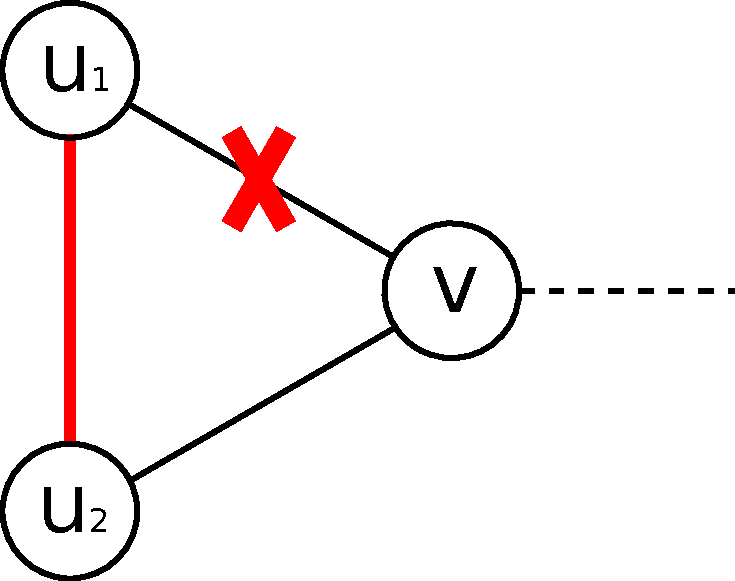
\includegraphics[width=0.3\textwidth]{images/pp_prevesenie.pdf}}

\caption[Prevesenie listového vrcholu]{Znázornenie operácie prevesenie listového vrchola
na iný list, s ktorým majú spoločného suseda. Táto operácia nezmenšuje počet vlastných
párov stromu.}

\label{pp:prevesenie}

\end{figure}

\begin{lema}
   Nech $T$ je strom, nech $u_1$ a $u_2$ sú listové vrcholy so spoločným susedom $v$. Potom
   $pp(T) \leq pp(T \cup (u_1, u_2) - (u_1, v))$. Táto grafová operácia je znázornená na
   obr. \ref{pp:prevesenie}.
\end{lema}

\begin{proof}
    Podobne ako v predošlej leme ukážeme, že každé $2$-pakovanie $S$ stromu $T$ je zároveň $2$-pakovaním
    v $T \cup (u_1, u_2) - (u_1, v)$. Nahliadneme, že zatiaľčo $d(u_1, u_2)$ klesne, vzdialenosť
    $u_1$ od akéhokoľvek iného vrcholu takouto výmenou neklesne. Zároveň sa nezmení vzdialenosť
    žiadnej inej dvojice vrcholov. Keďže $S$ nemôže obsahovať zároveň vrcholy $u_1$ aj $u_2$,
    vzdialenosť akejkoľvek dvojice vrcholov v $S$ touto operáciou neklesne, preto každá dvojica
    vrcholov v $S$ stále bude mať vzdialenosť aspoň $3$.
\end{proof}

Vďaka tejto leme sa pri dokazovaní horného ohraničenia počtu vlastných párov môžeme obmedziť
na stromy, ktorých žiadne dva listy nemajú spoločného suseda, okrem triviálneho prípadu
stromu s tromi vrcholmi.

Nech $T$ je strom s aspoň štyrmi vrcholmi, ktorého žiadne listy nemajú spoločný vrchol. Pozrieme
sa na najdlhšiu cestu $P$ v $T$. Koncový vrchol cesty označíme $v$, jeho suseda označíme $u$ a suseda $u$
iného, ako $v$ označíme $c$. Keďže žiaden vrchol nemá za susedov dva listy, $c$ je jednoznačne určený.
Ďalej sa v dôkaze horného ohraničenia rozoberá niekoľko prípadov podľa okolia vrchola $c$. Spomedzi
všetkých si ukážeme jeden, ostatné sa dajú vyriešiť podobným spôsobom.

Ak $\delta(c) = 2$, všetky vlastné páry $(S,X)$ rozdelíme na tie,
v ktorých $v$ patrí do $S$ a tie, kde $v$ nepatrí do $S$. Vlastných párov, kde $v$ nepatrí do $S$ je
dvakrát toľko ako v grafe $T - \{v\}$, podľa toho, či $v$ patrí do $X$. Tento počet vieme zhora
odhadnúť na $pp(n-1)$. Ak $v$ patrí do $S$, tak $u$ ani $c$ nemôžu patriť do $S$. Vlastných párov
v tomto prípade bude štornásobok počtu vlastných párov v grafe $T - \{v, u, c\}$, čo vieme zhora
odhadnúť ako $pp(n-3)$.

Dostávame teda nasledujúcu nerovnosť: $pp(n) \leq 2pp(n-1) + 4 pp(n-3)$. Vyriešením nerovností pre
všetky prípady dostaneme horné ohraničenie $pp(n) \leq 2 \tau^n$\cite{junosza_fast}, kde $\tau \approx 2.6488$ je kladný koreň rovnice
$$\tau^5 = 16\tau + 88.$$

\subsection{Dolné odhady hodnoty $pp(n)$}

\begin{figure}

\centerline{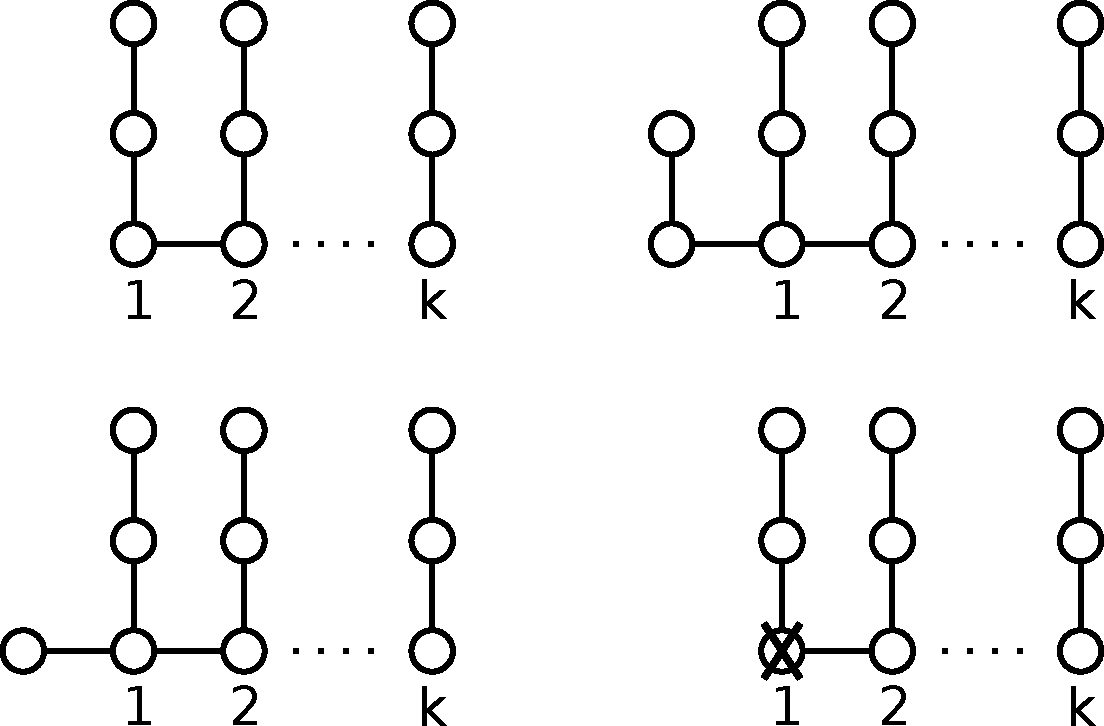
\includegraphics[width=0.8\textwidth]{images/pp_hreben.pdf}}

\caption[Trieda grafov s vysokým $pp(n)$]{Trieda grafov s $pp(n) = \Theta(2.6117^n)$}

\label{pp:hreben}

\end{figure}

Prvé dolné odhady hodnoty $pp(n)$ využívali grafy znázornené na obr. \ref{pp:hreben}.
Pomocou rekurzívneho vyjadrenia počtu vlastných párov na týchto špeciálnych grafoch
vzniklo dolné ohraničenie $pp(n) = \Omega(2.6117^n)$.

Analýzou zakorenených stromov s priemerom $6$ sa dá dolný odhad zvýšiť na $pp(n) = \Omega(2.6313^n)\cite{vlastne_pary}$.
Dôkladnejšou analýzou zakorenených stromov, ktorých všetky podstromy sú rovnaké, sa dá
odhad vylepšiť až na $pp(n) = \Omega(2.6391^n)$\cite{vlastne_pary}.
